\documentclass[a4paper,11pt]{article}

% --- PACKAGES ---
\usepackage[utf8]{inputenc}
\usepackage[T1]{fontenc}
\usepackage[english]{babel}
\usepackage{amsmath, amssymb, amsthm}
\usepackage{graphicx}
\usepackage{geometry}
\usepackage{hyperref}
\usepackage{subcaption}
\usepackage{float}
\usepackage{listings}
\usepackage{xcolor}
\usepackage{bm}
\usepackage{biblatex}

% --- SETUP MARGINI ---
\geometry{
    left=25mm,
    right=25mm,
    top=25mm,
    bottom=25mm
}

% --- SETUP LISTINGS ---
\definecolor{codegreen}{rgb}{0,0.6,0}
\definecolor{codegray}{rgb}{0.5,0.5,0.5}
\definecolor{codepurple}{rgb}{0.58,0,0.82}
\definecolor{backcolour}{rgb}{0.95,0.95,0.92}

\lstdefinestyle{mystyle}{
    backgroundcolor=\color{backcolour},   
    commentstyle=\color{codegreen},
    keywordstyle=\color{magenta},
    numberstyle=\tiny\color{codegray},
    stringstyle=\color{codepurple},
    basicstyle=\ttfamily\footnotesize,
    breakatwhitespace=false,         
    breaklines=true,                 
    captionpos=b,                    
    keepspaces=true,                 
    numbers=left,                    
    numbersep=5pt,                  
    showspaces=false,                
    showstringspaces=false,
    showtabs=false,                  
    tabsize=2,
    language=Matlab
}
\lstset{style=mystyle}

% --- COMANDI CUSTOM PER NOTAZIONE ---
\newcommand{\matr}[1]{\bm{#1}}     % Matrici in grassetto
\newcommand{\vect}[1]{\mathbf{#1}}  % Vettori/Punti in grassetto
\newcommand{\lineinf}{\ell_\infty}  % Linea all'infinito

% --- TITOLO ---
\title{
    \textbf{Image Analysis and Computer Vision} \\
    \large Homework Report
}
\author{Pietro Filippo Schgor \\ Person code: 10710527}
\date{\today}

\begin{document}

\maketitle

% --- 1. INTRODUZIONE ---
\section*{Part 1 - Theory}

% --- Q1 ---
\begin{figure}[h]
    \centering
    % --- First image (left) ---
    \begin{subfigure}[b]{0.45\textwidth}
        \centering
        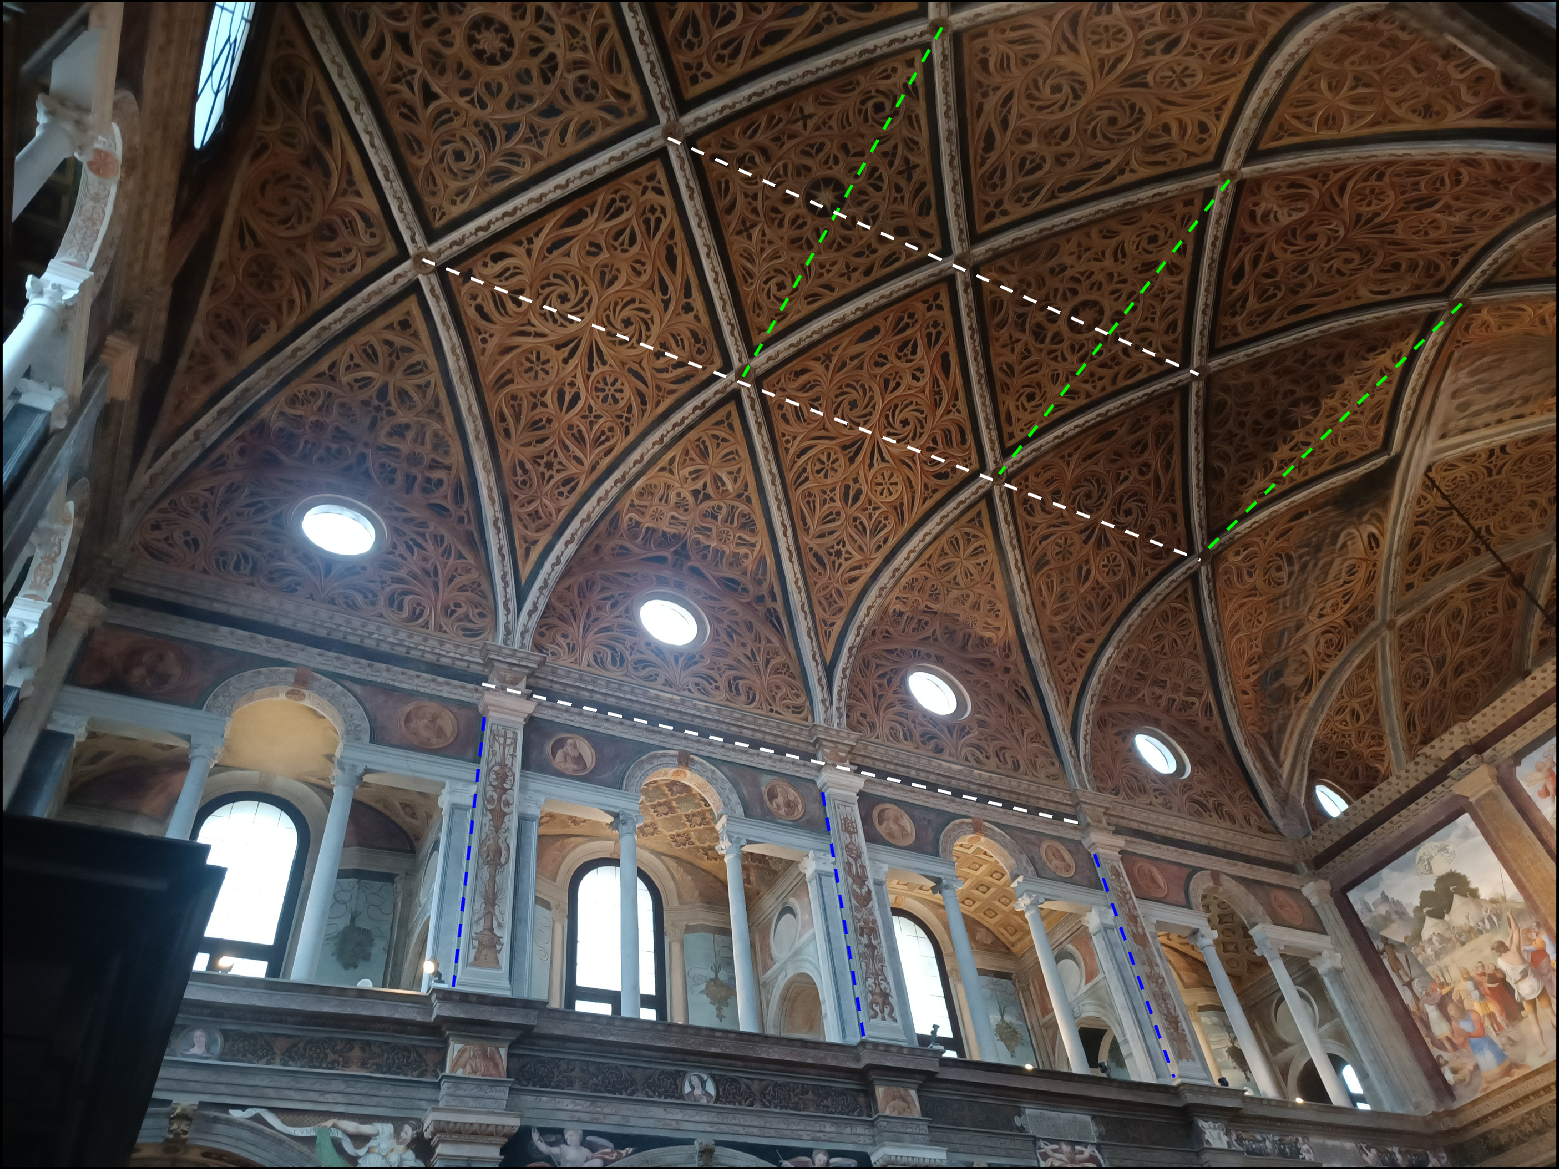
\includegraphics[width=\textwidth]{figures/given segments.png}
        \caption{}
        \label{fig:img1}
    \end{subfigure}
    \hfill % Pushes images to opposite sides
    % --- Second image (right) ---
    \begin{subfigure}[b]{0.45\textwidth}
        \centering
        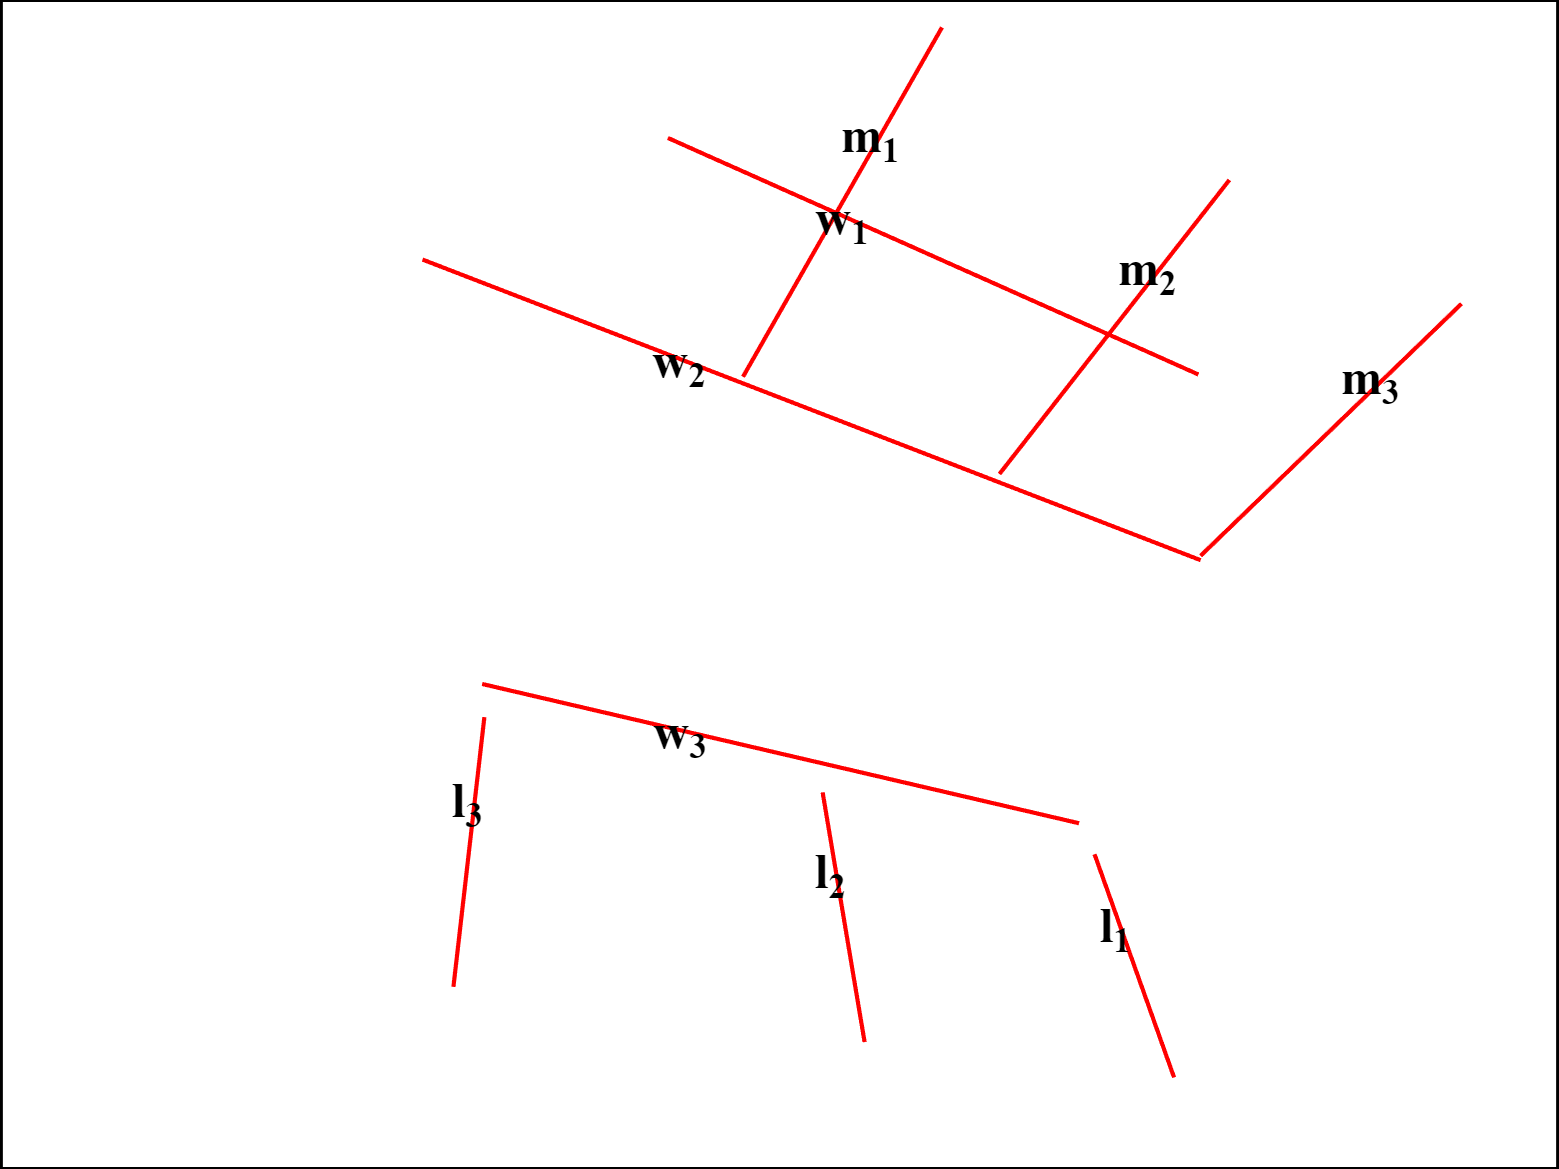
\includegraphics[width=\textwidth]{figures/extracted segments.png}
        \caption{ }
        \label{fig:img2}
    \end{subfigure}
    
    \caption{Given and extracted segments}
    \label{fig:due_immagini}
\end{figure}
\paragraph{Q1: From the above mentioned sets of lines, find the vanishing line $\ell'_{\infty}$ of any plane perpendicular to the cylinder Axis.}

\textbf{A1:} The vanishing line (horizon) is the image of the line at infinity $\lineinf$, representing the set of points at infinity. To identify the vanishing line of the plane perpendicular to the cylinder axis, we compute the vanishing points derived from sets of parallel lines in both the $X$ and $Y$ directions \ref{fig:due_immagini}:

\begin{itemize}
    \item $\vect{V}_x$ (Vanishing Point $X$): The intersection of the set of lines $\mathcal{L} = \{l_1, l_2, l_3\}$ parallel to the $X$-axis in 3D space.
    \item $\vect{V}_y$ (Vanishing Point $Y$): The intersection of the set of lines $\mathcal{M} = \{m_1, m_2, m_3\}$ parallel to the $Y$-axis in 3D space.
\end{itemize}

The line connecting $\vect{V}_x$ and $\vect{V}_y$ defines the vanishing line of the horizontal plane, denoted as $\ell'_\infty$:
\begin{equation}
    \ell'_\infty = \vect{V}_x \times \vect{V}_y = 
    \begin{bmatrix}
    a \\
    b \\
    c
    \end{bmatrix}
\end{equation}

% --- Q2 ---
\paragraph{Q2: Find the vanishing point in the direction of the cylinder axis.}

\textbf{A2:} As before, we compute the vanishing point in the direction of the cylinder axis as the intersection of a pair of lines parallel to the aforementioned axis.
Let $\vect{V}_z$ be the Vanishing Point $Z$: it is the intersection of the set of lines $\mathcal{W} = \{w_1, w_2, w_3\}$ parallel to the $Z$-axis in 3D space.

% --- Q3 ---
\paragraph{Q3: Using both the results of the previous points and the image of some of the diagonal arcs, find a (Euclidean) rectification mapping $\matr{H}_R$ for one of the vertical planes perpendicular to the cylinder axis. Compute the position of a non-apical nodal point on the chosen plane.}

\textbf{A3:} I chose the \textit{Stratified Rectification} method starting from the circular constraint, as there are not at least two non-parallel independent pairs of orthogonal lines available.

\begin{enumerate}
    \item \textbf{First step: Affine reconstruction (from Projective to Affine)} \\    We construct the affine mapping $\matr{H}_A$  that maps the imaged vanishing line $\ell'_\infty$ to the canonical line at infinity $\mathbf{l}_\infty = (0,0,1)^\top$:
    \begin{equation}
        \matr{H}_A = 
        \begin{bmatrix}
            1 & 0 & 0 \\
            0 & 1 & 0 \\
            a & b & c
        \end{bmatrix}, \matr{H}_A^{-T}\ell'_{\infty} = \mathbf{l}_\infty
    \end{equation}
    This transformation produces an image where the sets $\mathcal{L}$ and $\mathcal{M}$ become parallel. However, the image remains affinely distorted (angles are not preserved) \ref{fig:affine}.
     \begin{figure}[h]
    \centering
    % --- First image (left) ---
    \begin{subfigure}[b]{0.45\textwidth}
        \centering
        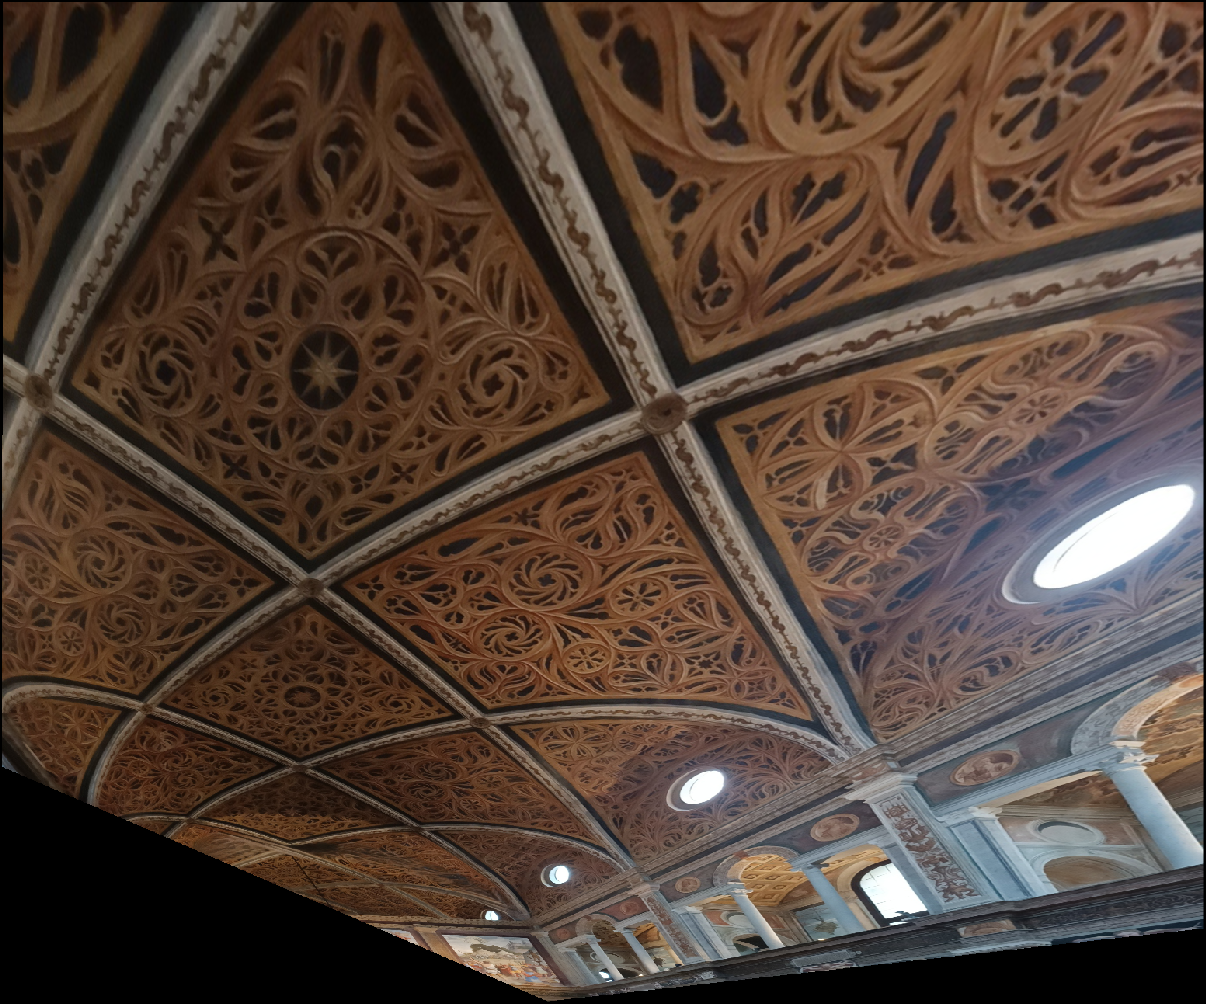
\includegraphics[width=\textwidth]{figures/affine rectification.png}
        \caption{Affine Rectification}
        \label{fig:affine}
    \end{subfigure}
    \hfill % Pushes images to opposite sides
    % --- Second image (right) ---
    \begin{subfigure}[b]{0.45\textwidth}
        \centering
        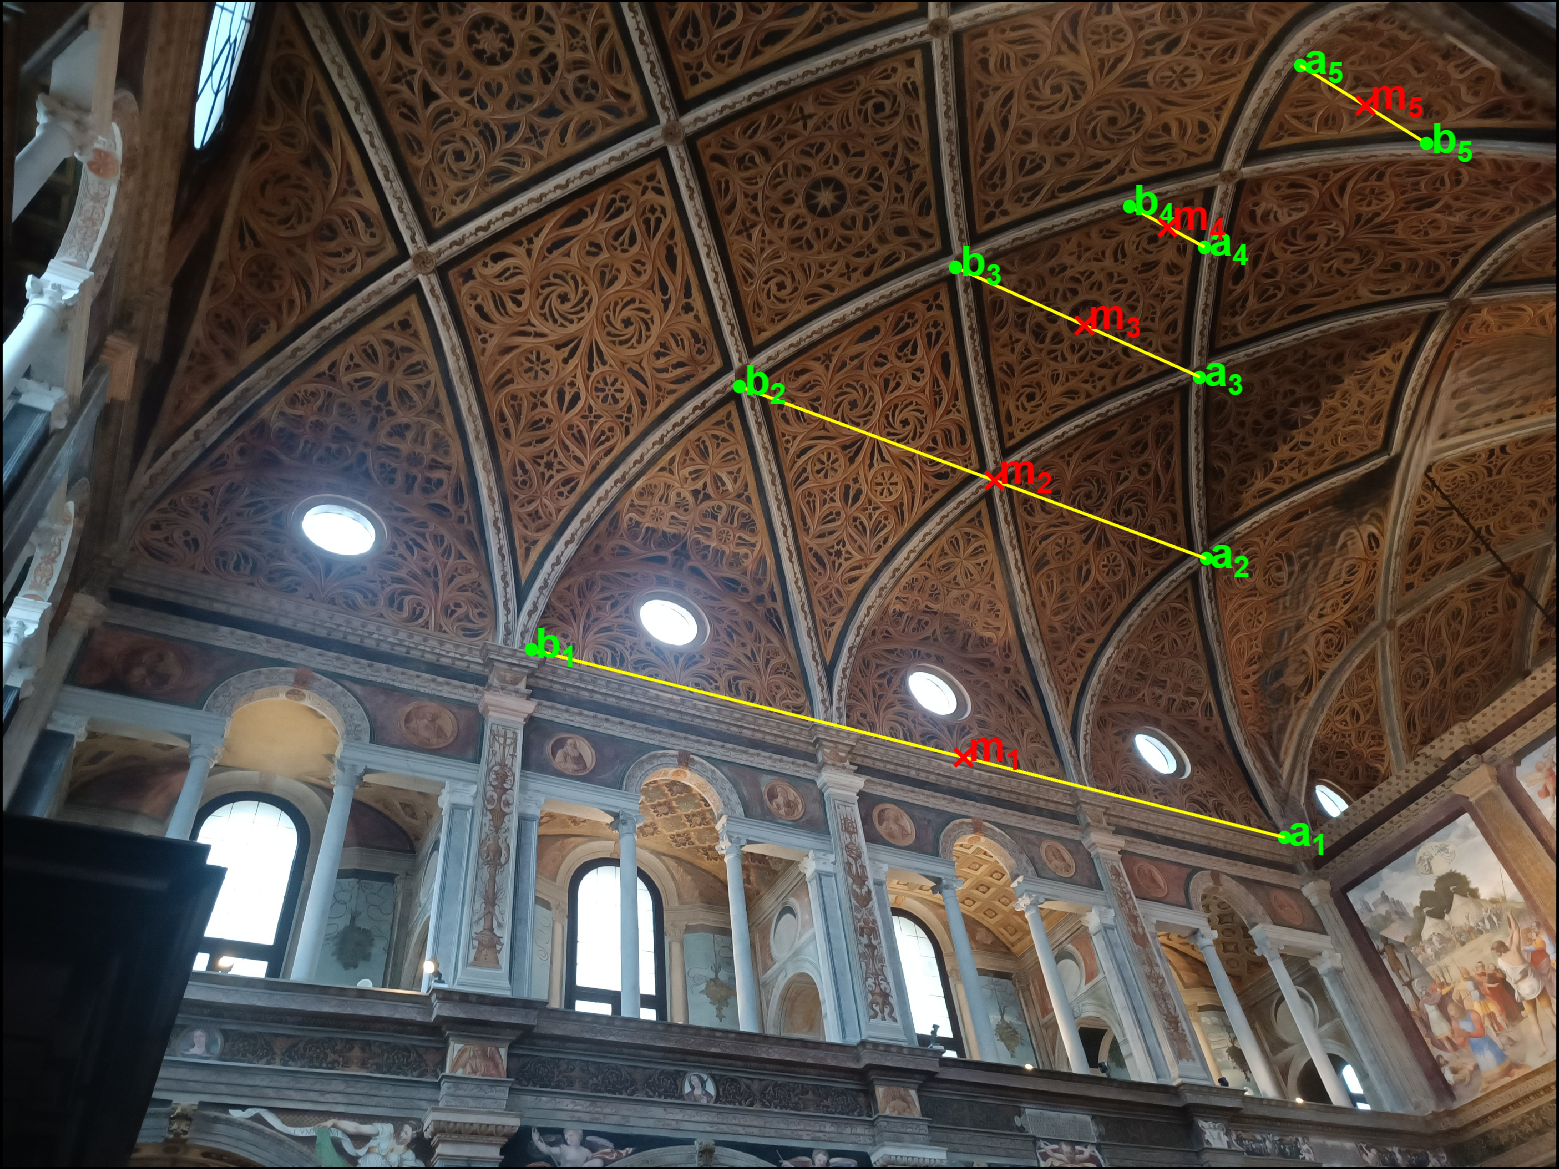
\includegraphics[width=\textwidth]{figures/5 midpoints.png}
        \caption{Midpoints }
        \label{Midpoints}
    \end{subfigure}
    
    \caption{ }
    \label{Q3}
\end{figure}
    
    \item \textbf{Second step: Shape reconstruction (from Affine to Metric)} \\
    We leverage the knowledge of the vault's geometry: the intersection of the cylindrical vault with a plane $X-Y$ perpendicular to the axis is a semicircle. We determine a second affine transformation $\matr{H}_B$ to rescale the rectified image, ensuring the axes of the circle are perpendicular and of equal length.

    \textbf{a) Feature Extraction (Harmonic Conjugates):}
Due to the symmetry of the diagonal arches, the midpoint of each pair of symmetric endpoints
$(a_i, b_i)$ \ref{Midpoints} lies on a plane perpendicular to the cylinder axis.
In the image, the midpoint $m_i$ is obtained as the harmonic conjugate of the vanishing point
$\vect{V}_z$ with respect to the points $a_i$ and $b_i$, satisfying the cross-ratio:
\[
(a_i, b_i; m_i, V_z) = -1
\]
This construction is invariant under projective transformations and allows the recovery of
the midpoints up to scale.

    
    \textbf{b) Conic Fitting:}
    We fit a conic section to these midpoints using the Direct Linear Transformation (DLT) method. The coefficient vector $\vect{c}$ minimizes $\|\matr{D}\vect{c}\|$ (via SVD) for the conic equation:
    \begin{equation}
        Ax^2 + Bxy + Cy^2 + Dx + Ey + F = 0
    \end{equation}
    Let $\matr{Q}$ be the matrix of the affine-rectified conic.
    
    \textbf{c) Metric Transformation Construction:}
    We extract the geometric properties of the ellipse from $\matr{Q}$: orientation $\alpha$, semi-major axis $a$, and semi-minor axis $b$. To restore circularity, we decompose the transformation $\matr{G}$ into rotation and isotropic scaling:
    
    Let $\matr{R}_{\alpha}$ be the rotation matrix and $\matr{S}$ the scaling matrix (with $\sigma = a/b$):
    \begin{equation}
        \matr{R}_{\alpha} = \begin{pmatrix} 
        \cos\alpha & -\sin\alpha \\ 
        \sin\alpha & \cos\alpha 
        \end{pmatrix}, \quad
        \matr{S} = \begin{pmatrix} 
        1 & 0 \\ 
        0 & \frac{a}{b} 
        \end{pmatrix}
    \end{equation}
    
    The local affine deformation $\matr{G}$ is:
    \begin{equation}
        \matr{G} = \matr{R}_{\alpha} \cdot \matr{S} \cdot \matr{R}_{\alpha}^T
    \end{equation}
    
    Embedding this into a homography $\matr{H}_B$:
    \begin{equation}
        \matr{H}_B = \begin{bmatrix} 
        G_{11} & G_{12} & 0 \\ 
        G_{21} & G_{22} & 0 \\ 
        0 & 0 & 1 
        \end{bmatrix} 
    \end{equation}
    
    The final Metric Rectification Homography $\matr{H}_R$ is:
    \begin{equation}
        \matr{H}_R = \matr{H}_B \cdot \matr{H}_A
    \end{equation}
\end{enumerate}

We can see that the resulting metric rectified image preserve angles and shape \ref{fig:metric}.

 \begin{figure}[h]
        \centering
        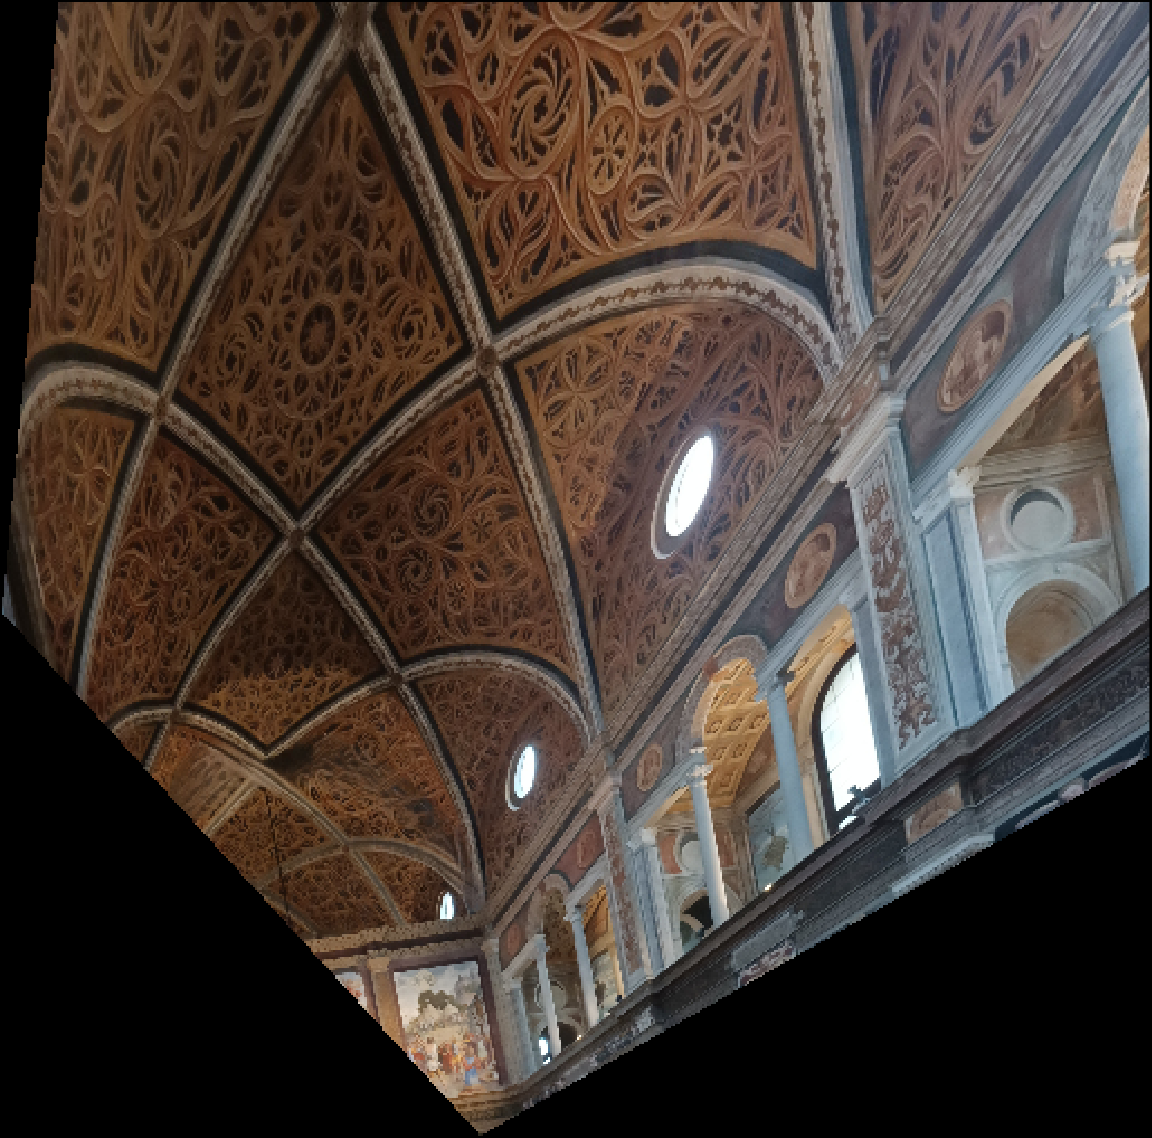
\includegraphics[width=0.45\textwidth]{figures/metric rectification.png}
        \caption{Metric Rectification}
        \label{fig:metric}
    \end{figure}
% --- Q4 ---

\paragraph{Q4: From the results of the previous points, compute the calibration matrix $\mathbf{K}$ of the camera.}

\textbf{A4:} 
The internal calibration of the camera is encapsulated in the matrix $\matr{K}$. To retrieve it, we estimate the \textit{Image of the Absolute Conic} (IAC), denoted as $\matr{\omega}$. The relationship is given by:
\begin{equation}
    \matr{\omega} = (\matr{K}\matr{K}^T)^{-1}
\end{equation}

We proceed with the assumption of \textbf{zero skew} ($s=0$), which implies that the camera sensor axes are orthogonal. The matrix $\matr{\omega}$ takes the following form:
\begin{equation}
    \matr{\omega} = 
    \begin{bmatrix}
    \omega_{11} & 0 & \omega_{13} \\
    0 & \omega_{22} & \omega_{23} \\
    \omega_{13} & \omega_{23} & \omega_{33}
    \end{bmatrix}
\end{equation}

To solve for the unknown entries of $\matr{\omega}$, we construct a linear system $\matr{A}\vect{w} = \vect{0}$ based on the geometric constraints of the scene:

\begin{enumerate}
    \item \textbf{Constraints from Rectifying Homography (Zhang's Constraints):} \\
    Let $\matr{H} = [\vect{h}_1, \vect{h}_2, \vect{h}_3]$ be the inverse of the rectification homography ($\matr{H} = \matr{H}_R^{-1}$). Since the rectification maps the image to a metric plane (where basis vectors are orthogonal and of equal length), the columns $\vect{h}_1$ and $\vect{h}_2$ must satisfy:
    \begin{align}
        \vect{h}_1^T \matr{\omega} \vect{h}_2 &= 0 \quad (\text{Orthogonality}) \\
        \vect{h}_1^T \matr{\omega} \vect{h}_1 - \vect{h}_2^T \matr{\omega} \vect{h}_2 &= 0 \quad (\text{Equal Magnitude})
    \end{align}
    The second constraint implicitly relates the scaling factors along the axes, allowing us to recover the aspect ratio ($f_x/f_y$) rather than assuming it.

    \item \textbf{Constraints from Vanishing Points (Pole-Polar relationship):} \\
    The vertical vanishing point $\vect{V}_z$ corresponds to the direction normal to the ground plane. In projective geometry, the vanishing point of the normal direction is the \textit{pole} of the vanishing line of the plane ($\vect{\ell}'_\infty$) with respect to the IAC:
    \begin{equation}
        \vect{\ell}'_\infty \propto \matr{\omega} \vect{V}_z
    \end{equation}
    This provides additional linear equations (via cross-product $(\matr{\omega} \vect{V}_z) \times \vect{\ell}'_\infty = \vect{0}$) to constrain the solution.
\end{enumerate}

\textbf{Solution and Extraction of K:} \\
The system is solved via Singular Value Decomposition (SVD) to find the parameter vector $\vect{w}$. Once $\matr{\omega}$ is reconstructed, the calibration matrix $\matr{K}$ is obtained via the inverse Cholesky decomposition ($\matr{\omega} = \matr{R}^T \matr{R} \implies \matr{K} = \matr{R}^{-1}$).
Finally, verifying the ratio $K_{11}/K_{22}$ allows us to discover that the pixels are indeed approximately square ($f_x \approx f_y$), validating the quality of the calibration.


% --- Q5 ---

\paragraph{Q5: Using the results of the previous points, choose one of the diagonal arcs and compute the 3D coordinates of a dozen of its points (e.g., w.r.t. a camera reference).}

\textbf{A5:} The 3D reconstruction is performed by exploiting the geometric relationship between two parallel diagonal arcs (ribs), denoted as arc $\mathcal{A}$ and arc $\mathcal{B}$, and the vanishing point of the cylinder axis $\vect{v}_z$.
Assuming a known Euclidean distance $d$ between the two parallel arcs (e.g., the distance between adjacent bays), we can triangulate the depth of corresponding points using the Law of Sines.

The procedure is as follows:
\begin{enumerate}
    \item \textbf{Back-projection:} Let $\vect{u}_A$ and $\vect{u}_B$ be the projections of corresponding points on the two arcs. We back-project them into unit viewing rays in the camera reference frame:
    \begin{equation}
        \vect{d}_A = \frac{\matr{K}^{-1}\vect{u}_A}{\|\matr{K}^{-1}\vect{u}_A\|}, \quad \vect{d}_B = \frac{\matr{K}^{-1}\vect{u}_B}{\|\matr{K}^{-1}\vect{u}_B\|}
    \end{equation}
    
    \item \textbf{Axis Direction:} The 3D direction of the cylinder axis (and thus the direction connecting the two parallel arcs) is given by the back-projection of the vanishing point $\vect{v}_z$:
    \begin{equation}
        \vect{n} = \frac{\matr{K}^{-1}\vect{v}_z}{\|\matr{K}^{-1}\vect{v}_z\|}
    \end{equation}
    
    \item \textbf{Triangulation (Law of Sines):} We solve the triangle formed by the camera center $O$ and the 3D points $A$ and $B$. We define the angles:
    \begin{equation}
        \theta = \arccos(\vect{d}_A \cdot \vect{d}_B), \quad \alpha = \arccos(\vect{d}_A \cdot \vect{n})
    \end{equation}
    The third angle is $\beta = \pi - (\theta + \alpha)$. Using the Law of Sines with the known baseline $d$:
    \begin{equation}
        \|A\| = d \cdot \frac{\sin(\beta)}{\sin(\theta)}, \quad \|B\| = d \cdot \frac{\sin(\alpha)}{\sin(\theta)}
    \end{equation}
    
    \item \textbf{3D Coordinates:} The final coordinates are obtained by scaling the viewing rays:
    \begin{equation}
        \vect{A}_{3D} = \|A\| \cdot \vect{d}_A
    \end{equation}
\end{enumerate}

% --- Q6 ---

\paragraph{Q6: Using $\matr{K}$, localize the cylinder axis w.r.t. the camera.}

\textbf{A6:} The cylinder axis is a 3D line parallel to the direction $\vect{n}$ (computed in A5) passing through the geometric center of the vault's cross-section.
To localize it, we combine the pole-polar relationship in the image plane with 3D plane intersection.

\begin{enumerate}
    \item \textbf{Image Center Localization:} The center of the circular cross-section in the image plane, denoted as $\vect{x}_c$, corresponds to the \textit{pole} of the vanishing line $\ell'_\infty$ with respect to the fitted conic $\matr{C}$ (from Q3). 
    \begin{equation}
        \vect{x}_c = \matr{C}^{-1} \ell'_\infty
    \end{equation}
    This point represents the projection of the axis centers at infinity.
    
    \item \textbf{Back-projection:} We generate the viewing ray $\vect{r}_c$ passing through the camera center and the image center $\vect{x}_c$:
    \begin{equation}
        \vect{r}_c = \matr{K}^{-1} \vect{x}_c
    \end{equation}
    The physical 3D axis must intersect this ray.
    
    \item \textbf{3D Anchor Point:} To resolve the scale ambiguity (i.e., where along the ray $\vect{r}_c$ the axis is located), we define a reference plane $\pi_{ref}$ passing through one of the reconstructed points from Q5 (e.g., the apex point $\vect{P}_{apex}$) and perpendicular to the axis direction $\vect{n}$. The plane equation is $\vect{n}^T (\vect{X} - \vect{P}_{apex}) = 0$.
    
    \item \textbf{Intersection:} The 3D center point $\vect{C}_{3D}$ is found by intersecting the ray $\vect{r}_c$ with the plane $\pi_{ref}$. Substituting $\vect{X} = \lambda \vect{r}_c$ into the plane equation:
    \begin{equation}
        \lambda = \frac{\vect{n}^T \vect{P}_{apex}}{\vect{n}^T \vect{r}_c} \implies \vect{C}_{3D} = \lambda \vect{r}_c
    \end{equation}
    
    \item \textbf{Axis Equation:} The cylinder axis is finally described as the line passing through $\vect{C}_{3D}$ with direction $\vect{n}$:
    \begin{equation}
        \mathcal{L}_{axis}(t) = \vect{C}_{3D} + t \cdot \vect{n}
    \end{equation}
\end{enumerate}

\section*{Part 2 - Matlab}

% --- Q1 ---
\paragraph{Q1: Feature Extraction}
The feature extraction was performed using a hybrid approach to ensure both efficiency and precision.
The image was first resized by a factor of 0.7 to reduce computational load.
\begin{itemize}
    \item \textbf{Lines for Vanishing Points:} The sets of lines $\mathcal{L}$, $\mathcal{M}$, and $\mathcal{W}$ were extracted using a semi-automatic helper function \texttt{extract\_lines}.
    \item \textbf{Midpoints for Conic Fitting:} A set of $N=12$ midpoints was manually selected using \texttt{ginput} to strictly define the geometry of the vault's cross-section. These points were saved to a \texttt{.mat} file to ensure reproducibility.
    \item \textbf{Arcs for 3D Reconstruction:} The corresponding points on the parallel diagonal arcs were manually selected to ensure correct correspondence between the two curves.
\end{itemize}

% --- Q2 ---
\paragraph{Q2: Implementation and Results}
The MATLAB script implements the geometric pipeline as follows:

\begin{itemize}
    \item \textbf{1-2. Vanishing Geometry:}
    The vanishing points $\vect{V}_x, \vect{V}_y, \vect{V}_z$ were computed using the MATLAB \texttt{cross} function on the homogeneous representations of the extracted lines.
    \begin{equation}
        \vect{V}_z = \begin{bmatrix} 6198.5 \\ 2474.4 \\ 1.000 \end{bmatrix}, \quad
        \ell'_\infty = \vect{V}_x \times \vect{V}_y = \begin{bmatrix} -0.0011 \\ -0.0003 \\ 1.0000 \end{bmatrix}
    \end{equation}

    \item \textbf{3. Rectification:}
    The affine rectification matrix $\matr{H}_A$ was constructed directly from the horizon line $\ell'_\infty$.
    For the metric rectification, we fitted a conic to the 12 selected midpoints. The fitting was performed using the \textbf{Direct Linear Transformation (DLT)} method, implemented via Singular Value Decomposition (\texttt{svd}) of the design matrix $\matr{D}$ containing terms $[x^2, xy, y^2, x, y, 1]$.
    The final rectification homography $\matr{H}_R$ was applied to the image using the \texttt{imwarp} function with a \texttt{projective2d} geometric transformation object.

    \item \textbf{4. Calibration:}
    The calibration matrix $\matr{K}$ was retrieved by solving for the Image of the Absolute Conic (IAC), $\omega$. We constructed a linear system $\matr{A}_{sys}\vect{w} = \mathbf{0}$ imposing:
    \begin{enumerate}
        \item Zhang's constraints (orthogonality and aspect ratio) derived from the columns of $\matr{H}_R^{-1}$.
        \item The pole-polar constraint relating the vertical vanishing point $\vect{V}_z$ and the horizon $\ell'_\infty$.
    \end{enumerate}
    The system was solved via \texttt{svd}. Since $\omega$ is positive-definite, $\matr{K}$ was extracted using the Cholesky factorization (\texttt{chol}):
    \[
    \matr{K} = \text{inv}(\text{chol}(\omega))
    \]
    The resulting calibration matrix (scaled by the image resize factor) is:
    \[
    \matr{K} =
    \begin{bmatrix}
    2131.47 & 0 & 1507.05 \\
    0 & 2131.47 & 1076.97 \\
    0 & 0 & 1
    \end{bmatrix}
    \]
    The principal point $(1507, 1077)$ is located near the center of the image, and the focal lengths are identical ($f_x = f_y$), confirming square pixels.

    \item \textbf{5. 3D Reconstruction:}
    The reconstruction was performed on 12 pairs of points from parallel diagonal arcs. We assumed a physical distance between the arcs of $d=2$ units (consistent with the MATLAB code).
    The points were back-projected into unit rays $\vect{d}_A, \vect{d}_B$ using $\matr{K}^{-1}$. The depth was calculated using the Law of Sines in a loop:
    \[
    \|A\| = d \cdot \frac{\sin(\beta)}{\sin(\theta)}
    \]
    where $\theta$ is the angle between the rays and $\beta$ is derived from the angle with the axis direction $\vect{n} = \matr{K}^{-1}\vect{V}_z$.
    The reconstructed coordinates for the selected arc are reported in Table \ref{tab:3d_points}.

    \begin{table}[H]
    \centering
    \caption{Reconstructed 3D coordinates of the arc (Sample of 12 points)}
    \label{tab:3d_points}
    \begin{tabular}{c r r r}
        \hline
        \textbf{Point} & \textbf{X} & \textbf{Y} & \textbf{Z} \\
        \hline
        1  & 0.0034 & 0.3357  & 3.6998 \\
        2  & 0.0499 & 0.1367  & 3.8859 \\
        3  & 0.1301 & -0.0126 & 3.9814 \\
        4  & 0.2582 & -0.1645 & 4.0926 \\
        5  & 0.3954 & -0.2958 & 4.1128 \\
        6  & 0.5686 & -0.4506 & 4.1867 \\
        7  & 0.7928 & -0.5800 & 4.2011 \\
        8  & 1.0165 & -0.6938 & 4.1842 \\
        9  & 1.2554 & -0.7891 & 4.1327 \\
        10 & 1.5479 & -0.8806 & 4.0263 \\
        11 & 1.8077 & -0.9435 & 3.9770 \\
        12 & 2.0721 & -0.9676 & 3.8430 \\
        \hline
    \end{tabular}
    \end{table}

    \item \textbf{6. Axis Localization:}
    The axis was localized by calculating the center of the cross-section in the image, $\vect{x}_c$, as the pole of the horizon line with respect to the conic $\matr{C}$.
    \[ \vect{x}_c = \matr{C}^{-1}\ell'_\infty \]
    This point was back-projected to a ray $\vect{r}_c$. The 3D center $\vect{CC}$ was found by intersecting $\vect{r}_c$ with the plane perpendicular to the axis direction passing through the 5th reconstructed point of the arc ($\vect{A}_5$).
    
    The resulting parametric equation of the axis is:
    \[
    \mathcal{L}_{axis}(t) = \begin{bmatrix} 1.1086 \\ -0.1790 \\ 2.4665 \end{bmatrix} + t \cdot \begin{bmatrix} 0.8787 \\ 0.2617 \\ 0.3992 \end{bmatrix}
    \]
\end{itemize}

\paragraph{Q3: 3D Visualization}
The following figures show the selected arc and the final 3D reconstruction viewed from four different perspectives to highlight the spatial structure of the vault.

\begin{figure}[H]
    \centering
    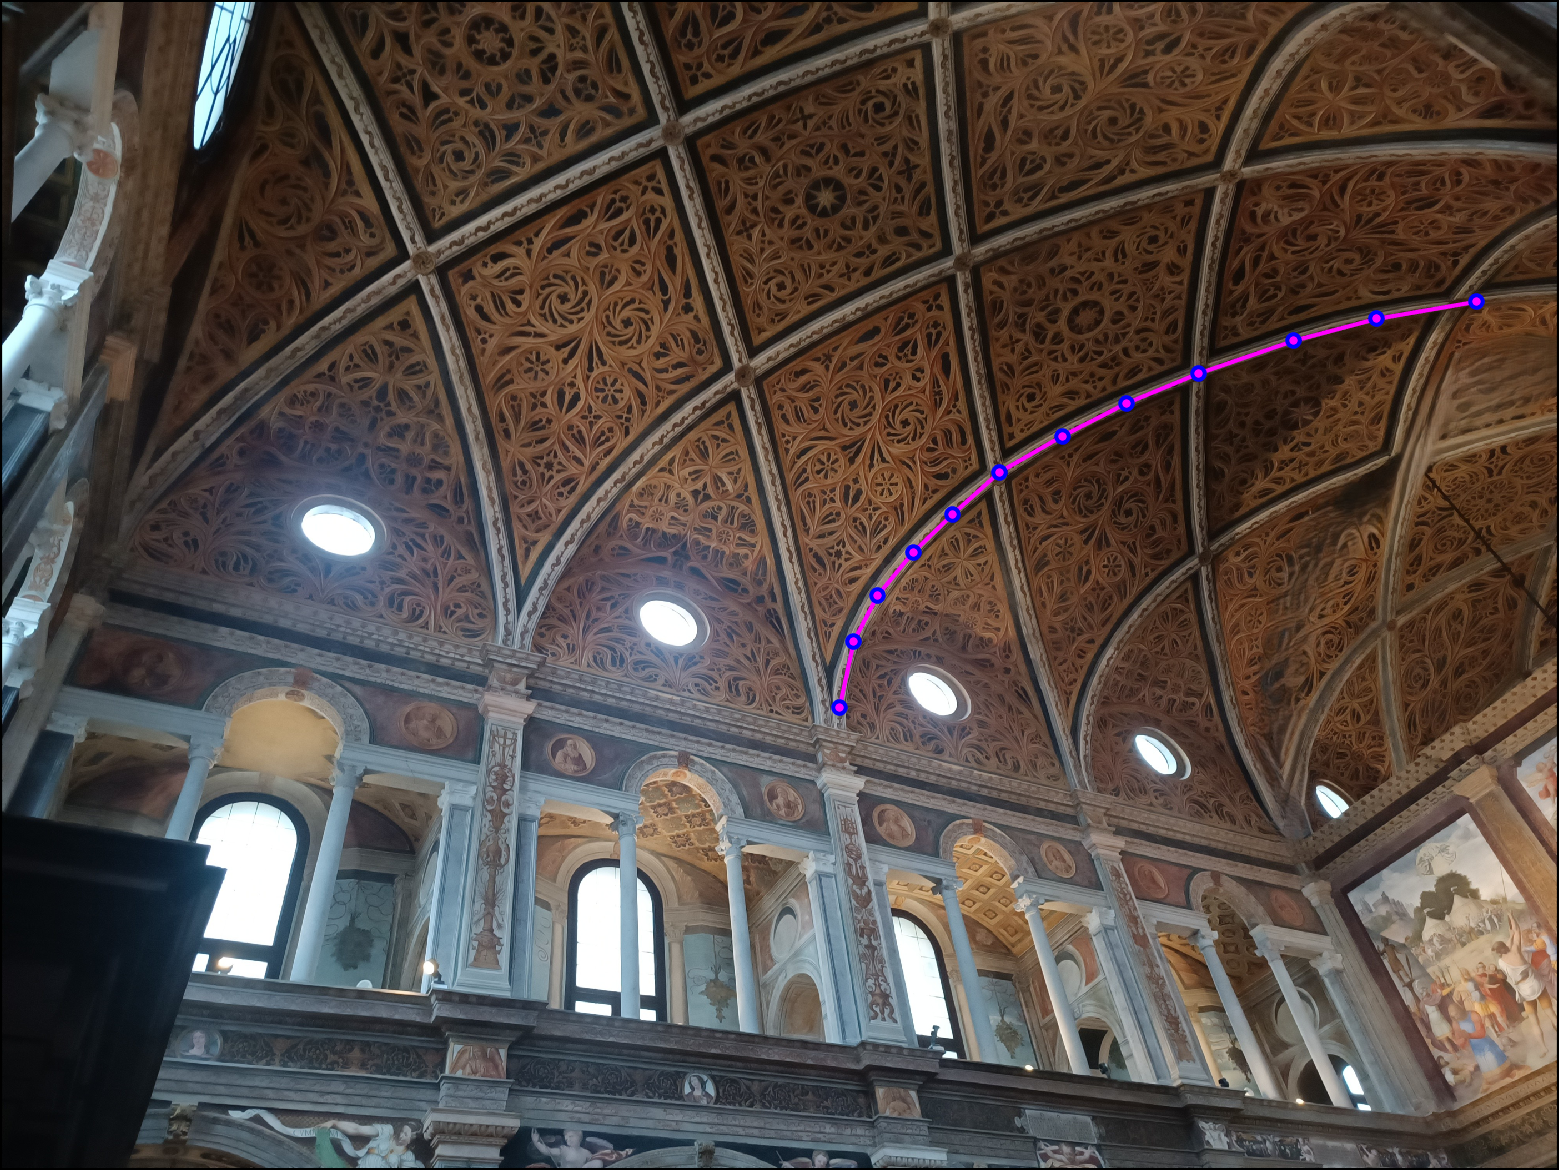
\includegraphics[width=0.6\textwidth]{figures/Selected Arc.png}
    \caption{Visualization of the extracted arc on the original image.}
    \label{fig:selected_arch}
\end{figure}

\begin{figure}[H]
    \centering
    \caption{Multi-view visualization of the 3D reconstructed arc, the camera position, and the cylinder axis.}
    \begin{subfigure}[b]{0.45\textwidth}
        \centering
        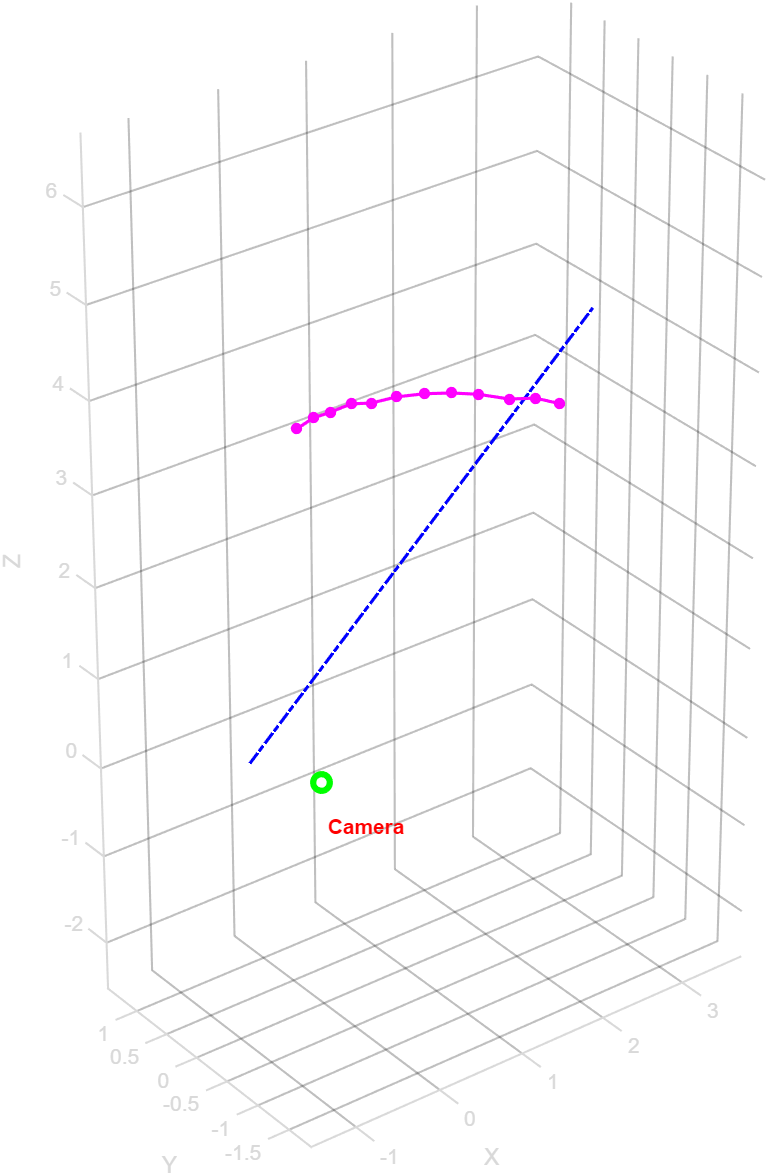
\includegraphics[width=\textwidth]{figures/3D Recon - Isometric View (Standard).png} 
        \caption{Isometric View}
    \end{subfigure}
    \hfill
    \begin{subfigure}[b]{0.45\textwidth}
        \centering
        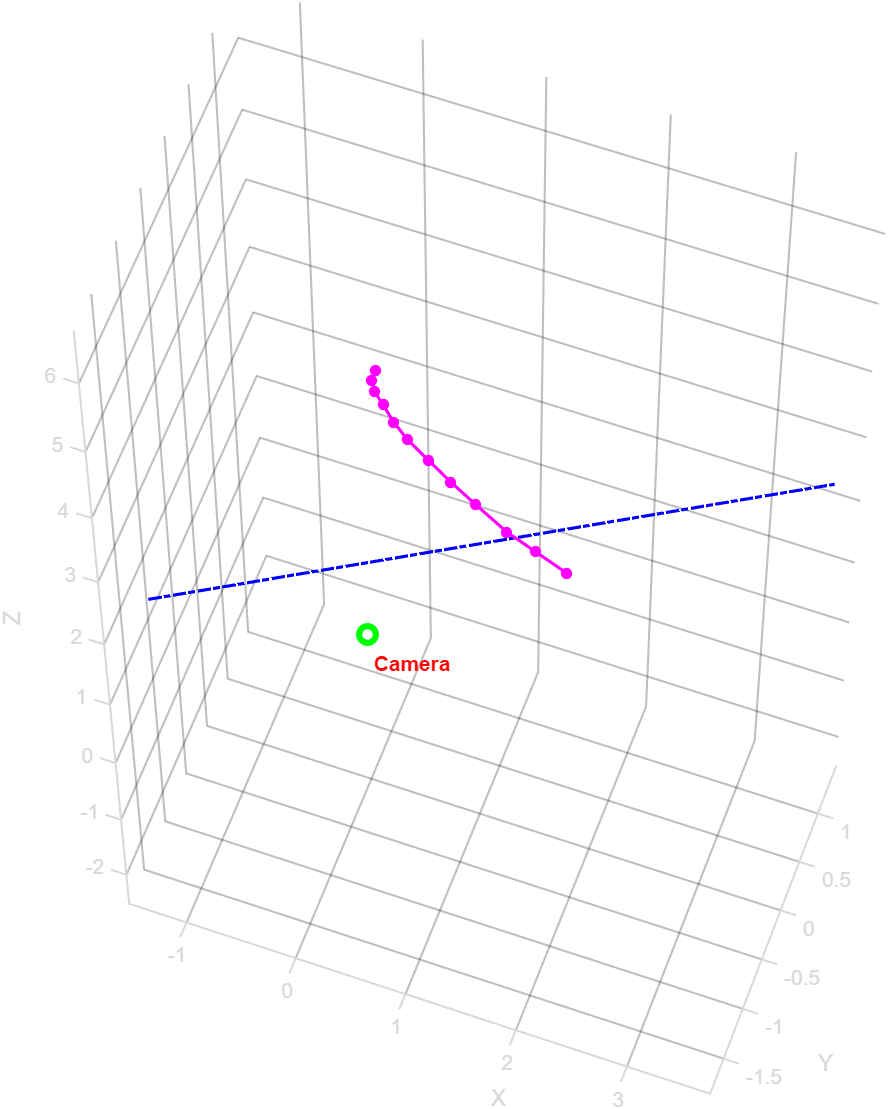
\includegraphics[width=\textwidth]{figures/3D Recon - High Angle (Bird's Eye).png}
        \caption{Bird's Eye View}
    \end{subfigure}
    
    \par\bigskip
    
    \begin{subfigure}[b]{0.45\textwidth}
        \centering
        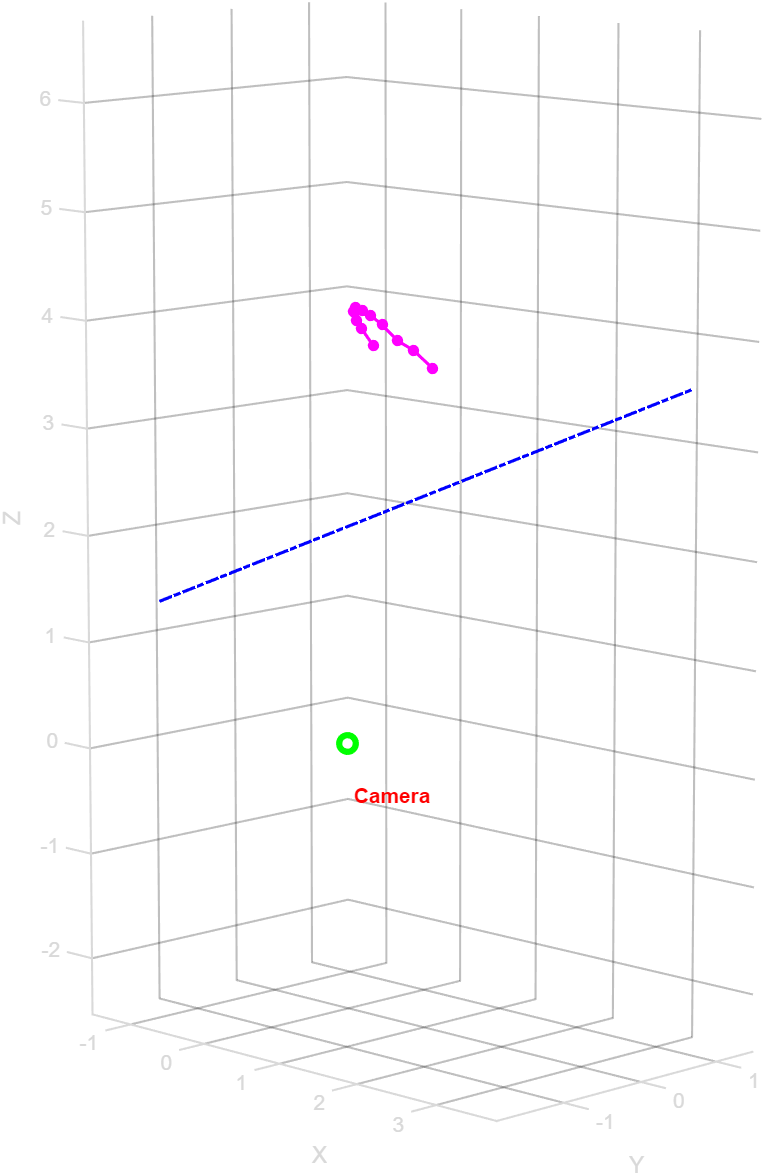
\includegraphics[width=\textwidth]{figures/3D Recon - Low Angle (Worm's Eye).png}
        \caption{Worm's Eye View}
    \end{subfigure}
    \hfill
    \begin{subfigure}[b]{0.45\textwidth}
        \centering
        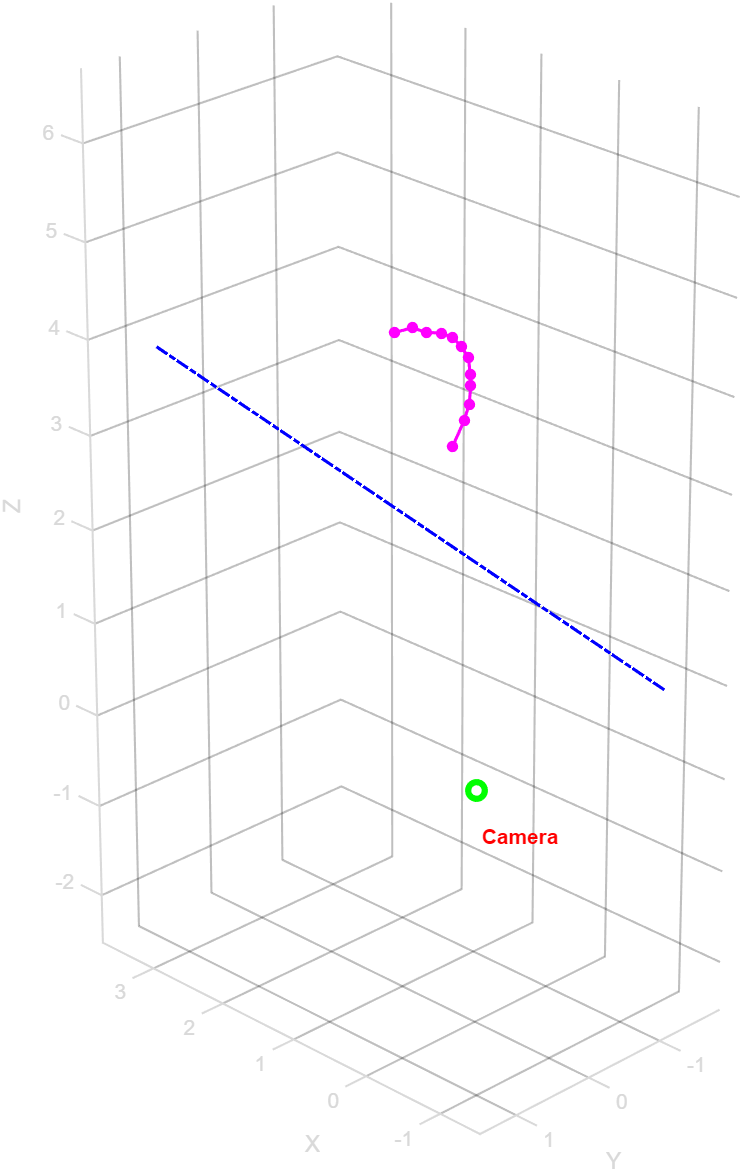
\includegraphics[width=\textwidth]{figures/3D Recon - Rear-Side View.png}
        \caption{Rear-Side View}
    \end{subfigure}
    
    
    \label{fig:3d_views}
\end{figure}
\end{document}